\chapter{Ergebnis} \label{summary}

\section{Der Gerippte} 
    Durch eine intensive Schlussphase konnten wir unsere drei anfänglich beschrieben Funktionen fertigstellen. (Siehe \ref{cpt:funktionen})

    Wir haben drei unserer Flaschenringfächern mit Sensoren ausgestattet um die Funktionalität vorzuführen, während alle Fächer mit jeweils 2 LEDs ausgestattet wurden. So konnten wir ebenfalls die ästhetische \enquote{Flaschen-Krone} präsentieren. Die weiß beleuchteten Flaschen haben den von uns erwünschten Eindruck erfüllt und es war ein belohnendes Gefühl den Flaschenring mit Flaschen zu füllen.

    Ebenfalls fertiggestellt haben wir den Einwurfsensor, welchen wir kurz vor der Präsentation in der AMD im vollständig zusammengesetzten Zustand erfolgreich testen und dem anwesenden Prof vorführen konnten.
    Als Antwort auf einen Einwurf konnten wir eine Animation über die gesamte Raute abspielen. Dabei ist uns aufgefallen, dass der obere der drei Kabelstränge beim Einbau trotz Heißklebepunkten auf den Kontakten ein Wackelkontakt entwickelt hat, der die drei Farbwerte aus der Synchronität bringt. Da wir den Ursprung in der verleibenden Zeit nicht finden konnten, mussten wir uns entscheiden, nur eine der drei Farbkanäle anzusteuern. So haben wir uns für blaue Animationen entschieden.

    Ein weiteres Problem ist beim Abbau der Tonne für den Transport aufgetreten. Beim herausnehmen der inneren Tonne gab es erneut Probleme mit den LED-Strips. Diesmal gab es im unteren Kabelstrang Kontakt zwischen Strom und Erdung eine Verbindung, wodurch der LED-Strip extrem heiß wurde. Auch hier konnten wir leider keine Fehleranalyse mehr durchführen und mussten den unteren Teil für die anstehende Präsentation ausstecken.

    Auch erfolgreich umgesetzt haben wir die kleinen Rauten-Modelle, die andere Mülleimer simulieren sollten. Hier haben wir die Kommunikation zwischen dem Hauptmodell und einer Raute und parallel zwischen dem Hauptmodell und einem Handy, das die zweite Raute simuliert hat, mit dem in \ref{sec:communications} beschriebenem Ansatz getestet. Wir haben es aber nicht hinbekommen, beide Rauten anzuspielen. Den genauen Grund konnten wir uns, ebenfalls wegen der kurzen Zeit zur Abschlussveranstaltung, nicht mehr rekonstruieren.

    \begin{figure}[H]
        \begin{center}
            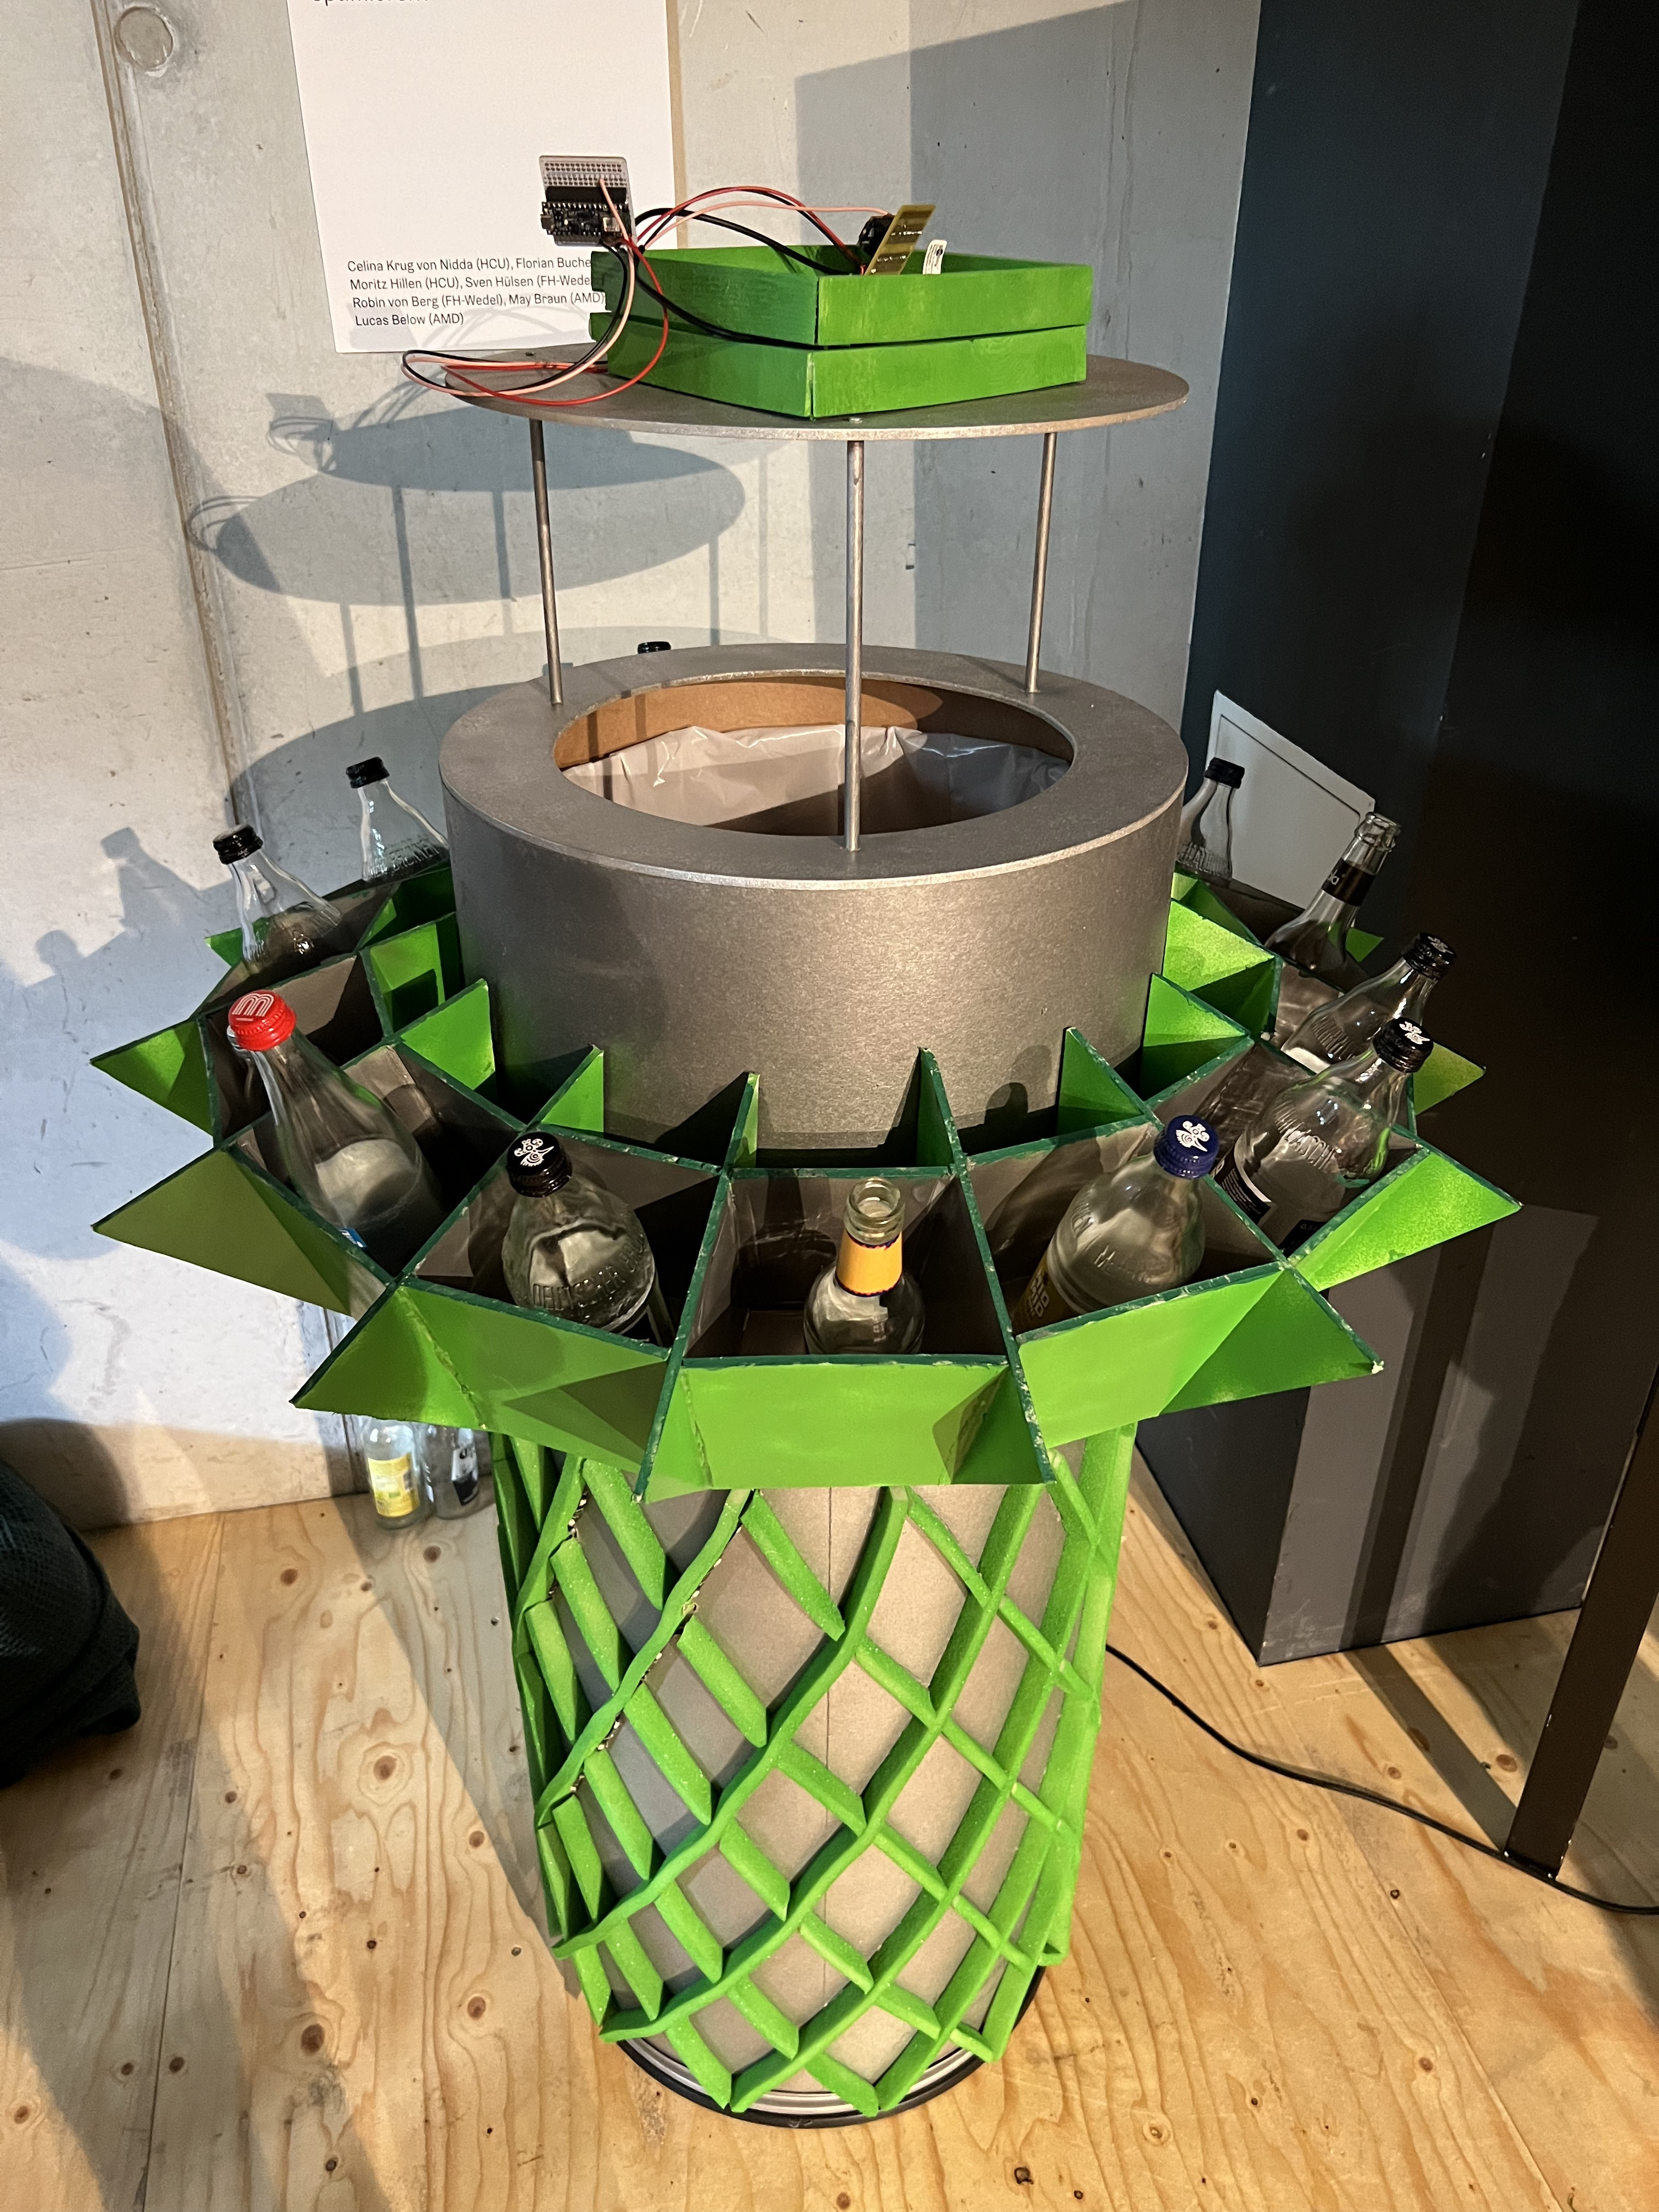
\includegraphics[width=6cm]{media/04_result/pic_bin.jpg}
        \end{center}
        \caption{Der Gerippte bei der Abschlussveranstaltung im betahaus mit den beiden Rauten auf dem Deckel.}
        \label{fig:pic_gerippte_1}
    \end{figure}

\section{Abschlussveranstaltung}

    \begin{figure}[H]
        \begin{subfigure}[b]{0.5\textwidth}
            \centering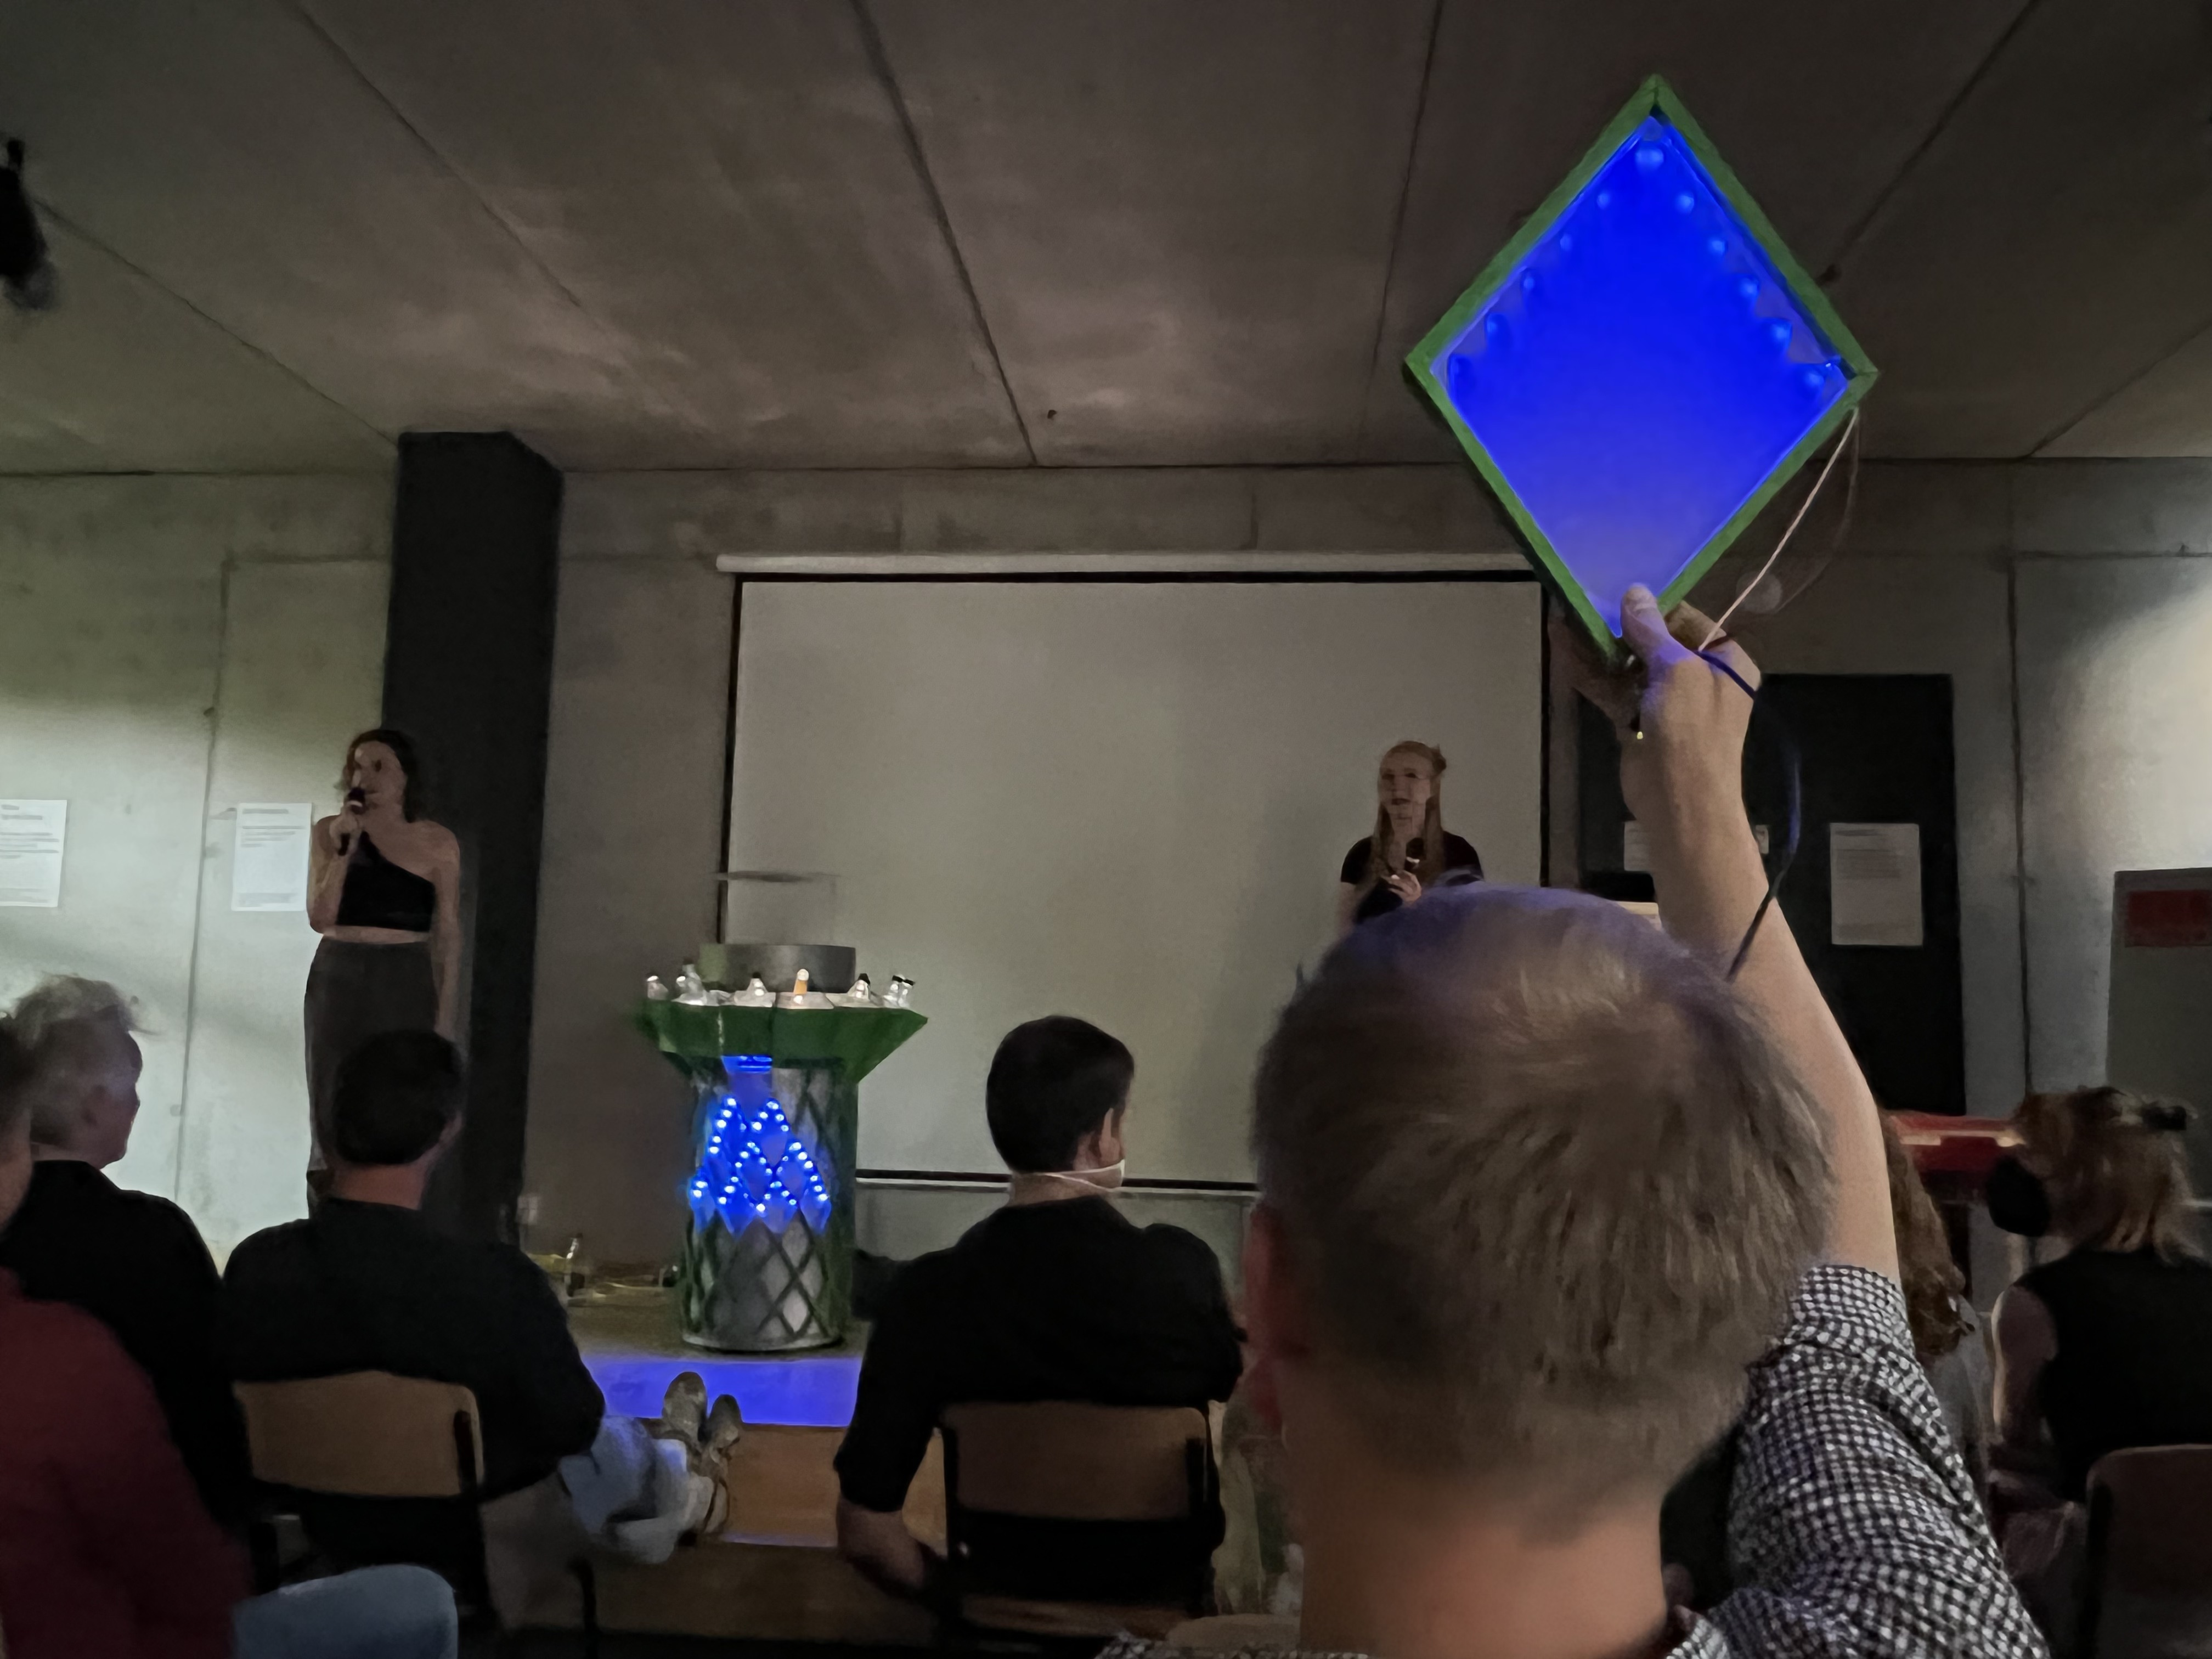
\includegraphics[width=\textwidth]{media/04_result/pic_communication.jpg}
            \caption{Unser Rauten-Modell in Aktion.}
            \label{fig:pic_gerippte_2}
        \end{subfigure}\quad
        \begin{subfigure}[b]{0.5\textwidth}
            \centering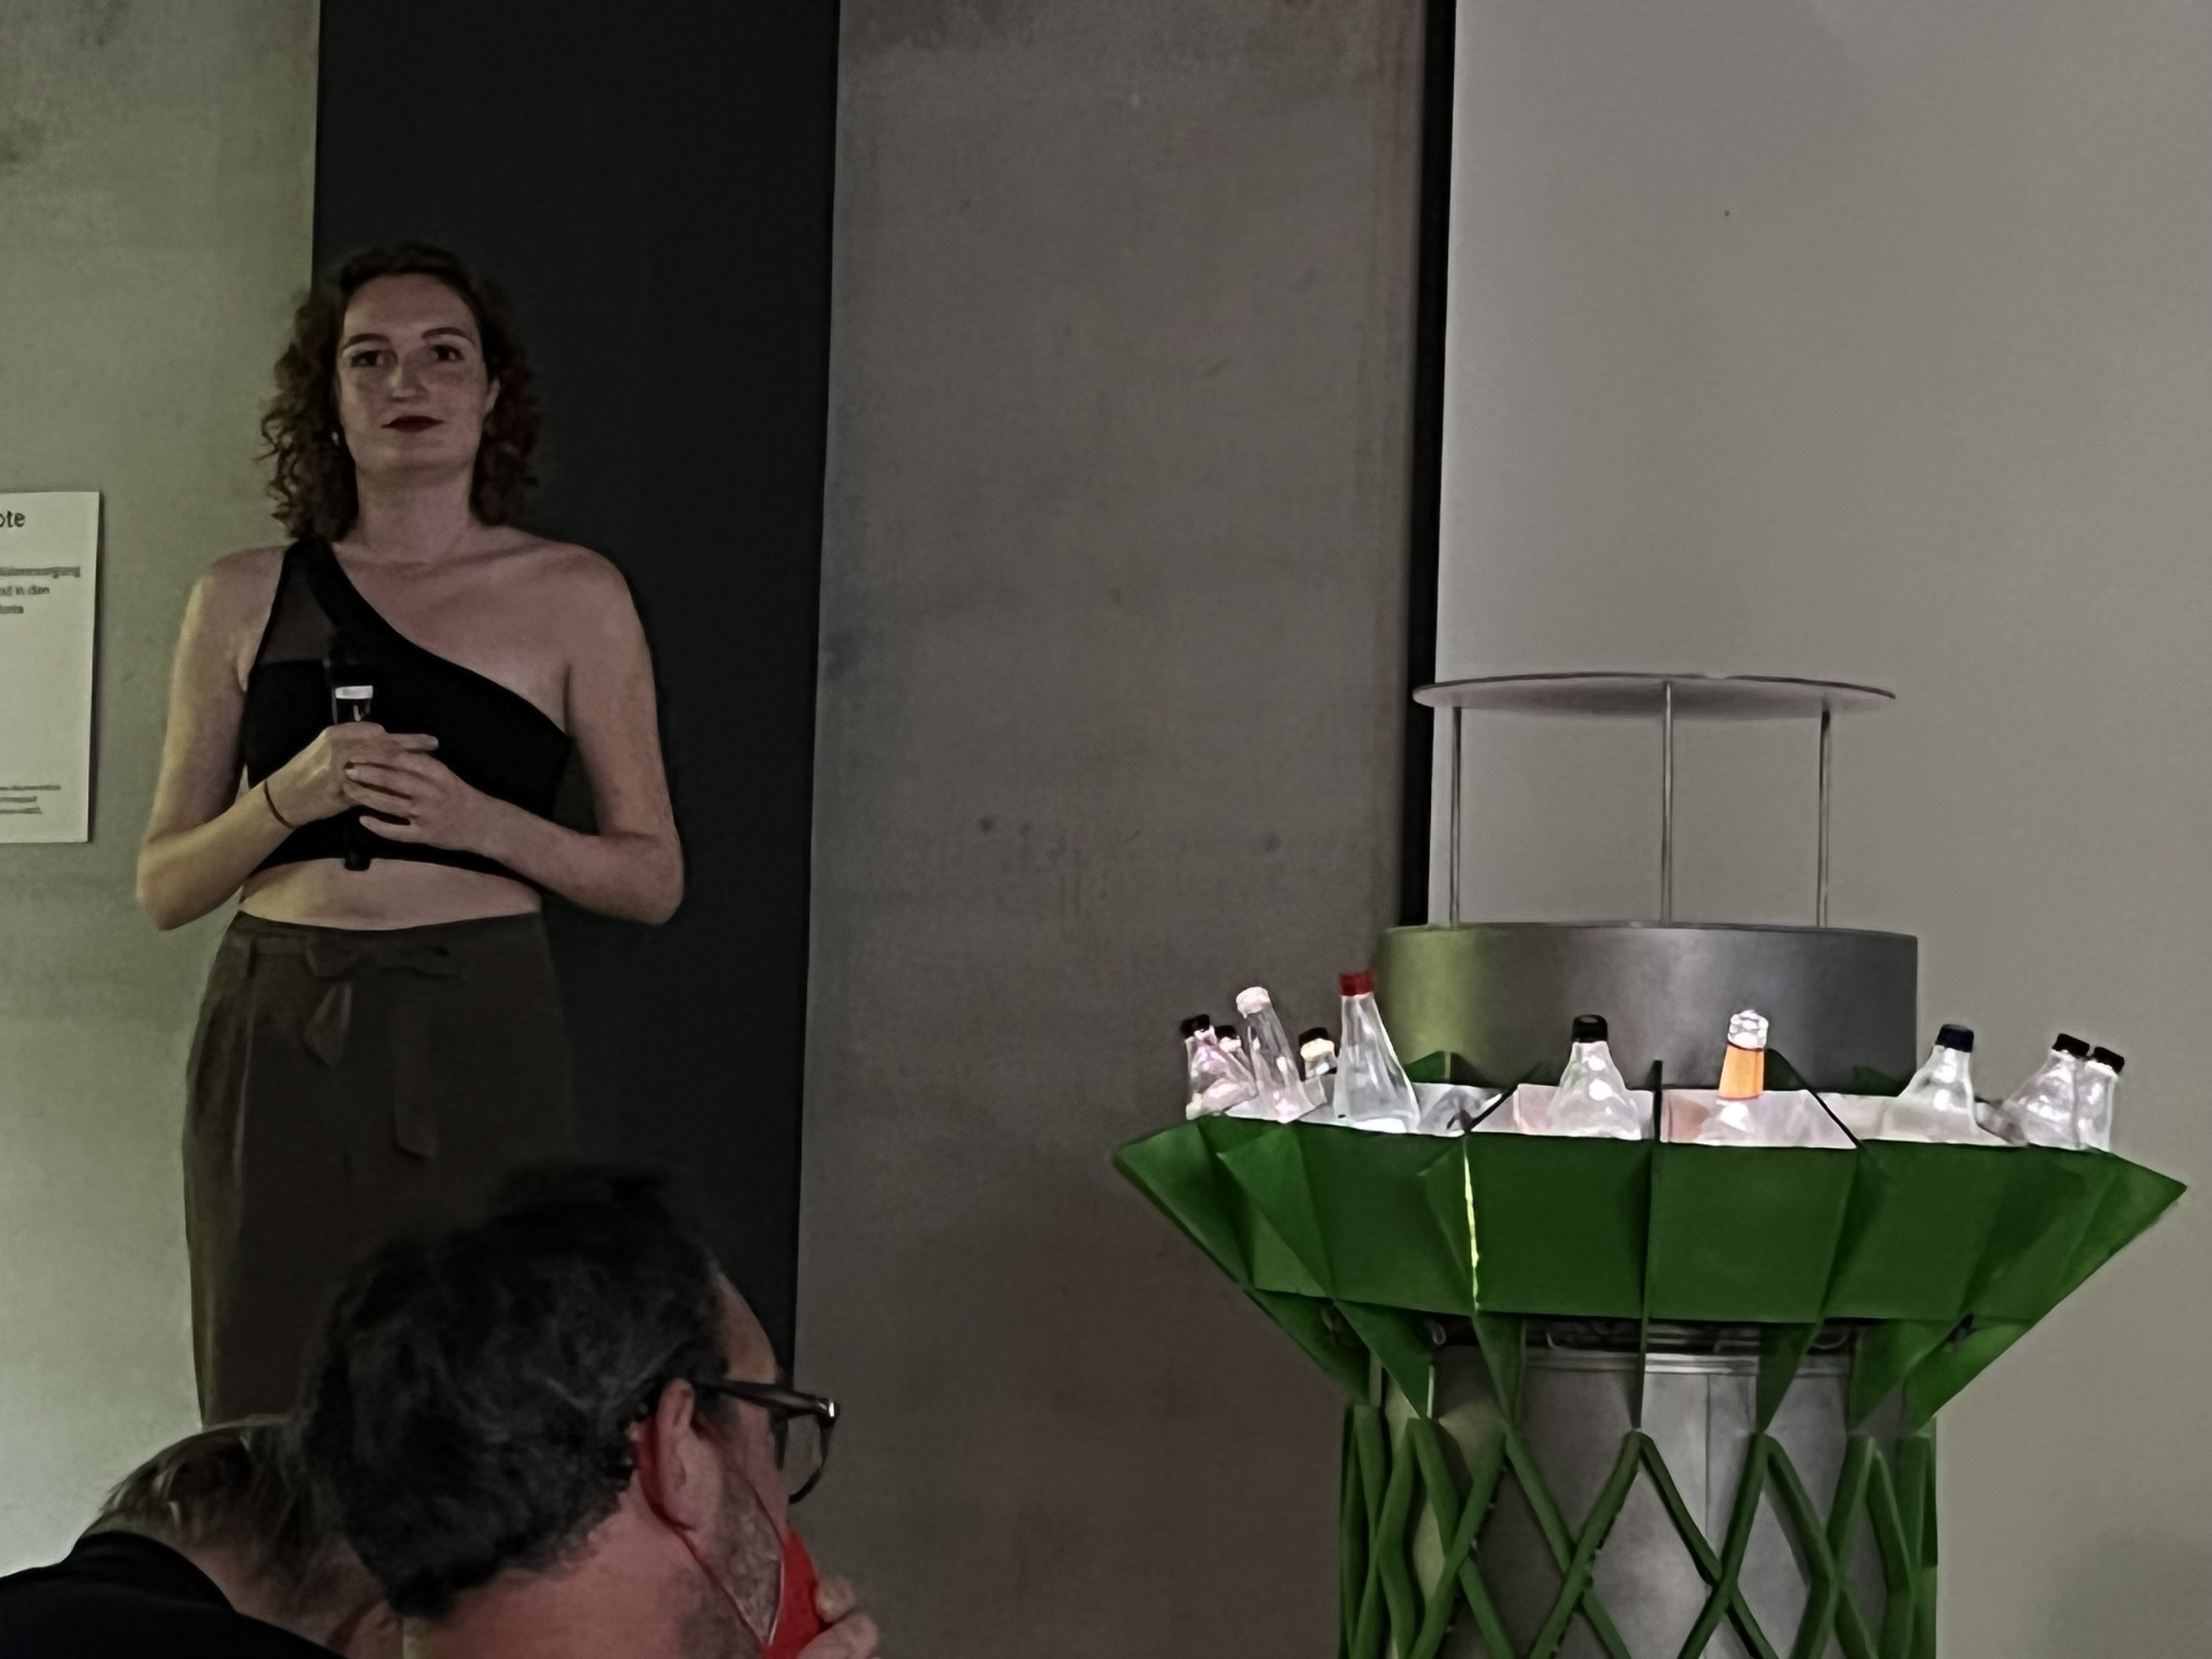
\includegraphics[width=0.7\textwidth]{media/04_result/pic_presentation_bottles.jpg}
            \caption{Beleuchtung der Flaschen im Flaschenring.}
            \label{fig:pic_gerippte_3}
        \end{subfigure}
        \caption{Eindrücke aus dem Pitch der Abschlussveranstaltung}
    \end{figure}

    Die im betahaus stattfindende Veranstaltung hat am \printdate{2022-06-30} um 18 Uhr stattgefunden. Hier haben alle 5 Teams ihre Modelle und Konzepte in einem sieben minütigem Pitch vorgestellt. Für unser Team haben Celina Krug und Maybritt Braun einen Pitch mit Unterstützung des Teams vorbereitet und dort hervorragend vorgetragen. Trotz eines unglücklichem Umstands, der Einwurfsensor hat, nachdem er vorher Vorort getestet wurde, während der Vorstellung dauerhaft ausgelöst, was unsere Funktionalität leider viel einfacher dargestellt hat, als sie im Hintergrund ablief.
    Der Grund der Fehlauslösungen liegt höchstwahrscheinlich in der Konfiguration des Sensors, denn auch wenn der maximale Abstand geringer eingestellt war, als die Kantenlänge des Sensorbereichs, kann es sein, dass diese Konfiguration im Sensor nicht fein genug umgesetzt werden kann und wir eine geringere Reichweite Wählen müssen.
        